\documentclass{tufte-handout}

\usepackage{amsmath}
\usepackage{graphicx}
\setkeys{Gin}{width=\linewidth,totalheight=\textheight,keepaspectratio}

\usepackage{booktabs}
\usepackage{units}
\usepackage{fancyvrb}
\fvset{fontsize=\normalsize}
\usepackage{multicol}
\usepackage{lipsum}
\PassOptionsToPackage{dvipsnames}{xcolor}
\usepackage{xcolor}
\usepackage{amsmath, amsthm, thmtools}
\usepackage{amssymb}
\usepackage{cleveref}
\usepackage{csquotes}
\geometry{
  marginparwidth=60mm % width of margin notes
}
%%%%%%%%% mathematical bold  %%%%%%%%%%%%%%%%%

\newcommand{\bA}{\mathbb{A}}
\newcommand{\bB}{\mathbb{B}}
\newcommand{\bC}{\mathbb{C}}
\newcommand{\Cs}{\bC^\times}
\newcommand{\bD}{\mathbb{D}}
\newcommand{\bE}{\mathbb{E}}
\newcommand{\F}{\mathbb{F}}
\newcommand{\bF}{\mathbb{F}}
\newcommand{\bG}{\mathbb{G}}
\newcommand{\bH}{\mathbb{H}}
\newcommand{\bI}{\mathbb{I}}
\newcommand{\bJ}{\mathbb{J}}
\newcommand{\bK}{\mathbb{K}}
\newcommand{\bL}{\mathbb{L}}
\newcommand{\bM}{\mathbb{M}}
\newcommand{\N}{\mathbb{N}}
\newcommand{\bO}{\mathbb{O}}
\newcommand{\bP}{\mathbb{P}}
\newcommand{\bp}{\mathbb{p}}
\newcommand{\Q}{\mathbb{Q}}
\newcommand{\R}{\mathbb{R}}
\newcommand{\bS}{\mathbb{S}}
\newcommand{\bT}{\mathbb{T}}
\newcommand{\bU}{\mathbb{U}}
\newcommand{\bV}{\mathbb{V}}
\newcommand{\bW}{\mathbb{W}}
\newcommand{\bX}{\mathbb{X}}
\newcommand{\bY}{\mathbb{Y}}
\newcommand{\Z}{\mathbb{Z}}

%%%%%%%%% calligraphic %%%%%%%%%%%%%%%%%%%%%%%

\newcommand{\mc}[1]{\mathcal{#1}}
\newcommand{\cA}{\mathcal{A}}
\newcommand{\cB}{\mathcal{B}}
\newcommand{\cC}{\mathcal{C}}
\newcommand{\cD}{\mathcal{D}}
\newcommand{\cE}{\mathcal{E}}
\newcommand{\cF}{\mathcal{F}}
\newcommand{\cG}{\mathcal{G}}
\newcommand{\cH}{\mathcal{H}}
\newcommand{\cI}{\mathcal{I}}
\newcommand{\cJ}{\mathcal{J}}
\newcommand{\cK}{\mathcal{K}}
\newcommand{\cL}{\mathcal{L}}
\newcommand{\cM}{\mathcal{M}}
\newcommand{\cm}{\mathcal{m}}
\newcommand{\cN}{\mathcal{N}}
\newcommand{\cO}{\mathcal{O}}
\newcommand{\cP}{\mathcal{P}}
\newcommand{\cQ}{\mathcal{Q}}
\newcommand{\cR}{\mathcal{R}}
\newcommand{\cS}{\mathcal{S}}
\newcommand{\cT}{\mathcal{T}}
\newcommand{\cU}{\mathcal{U}}
\newcommand{\cV}{\mathcal{V}}
\newcommand{\cW}{\mathcal{W}}
\newcommand{\cX}{\mathcal{X}}
\newcommand{\cY}{\mathcal{Y}}
\newcommand{\cZ}{\mathcal{Z}}

%%%%%%%%% mathematical fraktur  %%%%%%%%%%%%%%

\newcommand{\mf}[1]{\mathfrak{#1}}
\newcommand{\fa}{\mathfrak{a}}
\newcommand{\fb}{\mathfrak{b}}
\newcommand{\fc}{\mathfrak{c}}
\newcommand{\fA}{\mathfrak{A}}
\newcommand{\fB}{\mathfrak{B}}
\newcommand{\fC}{\mathfrak{C}}
\newcommand{\fD}{\mathfrak{D}}
\newcommand{\fE}{\mathfrak{E}}
\newcommand{\fF}{\mathfrak{F}}
\newcommand{\fG}{\mathfrak{G}}
\newcommand{\fH}{\mathfrak{H}}
\newcommand{\fI}{\mathfrak{I}}
\newcommand{\fJ}{\mathfrak{J}}
\newcommand{\fK}{\mathfrak{K}}
\newcommand{\fL}{\mathfrak{L}}
\newcommand{\fm}{\mathfrak{m}}
\newcommand{\fN}{\mathfrak{N}}
\newcommand{\fO}{\mathfrak{O}}
\newcommand{\fp}{\mathfrak{p}}
\newcommand{\fQ}{\mathfrak{Q}}
\newcommand{\fq}{\mathfrak{q}}
\newcommand{\fR}{\mathfrak{R}}
\newcommand{\fS}{\mathfrak{S}}
\newcommand{\fT}{\mathfrak{T}}
\newcommand{\fU}{\mathfrak{U}}
\newcommand{\fV}{\mathfrak{V}}
\newcommand{\fW}{\mathfrak{W}}
\newcommand{\fX}{\mathfrak{X}}
\newcommand{\fY}{\mathfrak{Y}}
\newcommand{\fZ}{\mathfrak{Z}}

%%%%%%%%%    math operators    %%%%%%%%%%%%%%%

\newcommand{\RP}{\mathbb{RP}}
\newcommand{\gen}[1]{\langle #1\rangle}
\newcommand{\Id}{\mathrm{Id}}
\DeclareMathOperator{\im}{im}
\DeclareMathOperator{\ggt}{ggT}
\DeclareMathOperator{\kgv}{kgV}
\DeclareMathOperator{\Aut}{Aut}
\DeclareMathOperator{\Hom}{Hom}
\DeclareMathOperator{\Iso}{Iso}
\DeclareMathOperator{\ord}{ord}
\DeclareMathOperator{\rad}{rad}
\DeclareMathOperator{\GL}{GL}
\DeclareMathOperator{\SL}{SL}
\DeclareMathOperator{\UT}{UT_3(\R)}
\DeclareMathOperator{\id}{id}
\DeclareMathOperator{\sgn}{sgn}
\DeclareMathOperator{\modn}{mod}
\DeclareMathOperator{\stab}{Stab_G}
\DeclareMathOperator{\Th}{Th}
\DeclareMathOperator{\On}{On}
\DeclareMathOperator{\Spec}{Spec}
\DeclareMathOperator{\coker}{coker}

%%%%%%%%%    further commands  %%%%%%%%%%%%%%%

\DeclareMathOperator{\nil}{nil}
\DeclareMathOperator{\Jac}{Jac}
\setlength{\headheight}{13.59999pt}

%%%%%%%%%    thmtools environments  %%%%%%%%%%%%%%%

\declaretheoremstyle[
shaded={
    rulecolor=Lavender!35,
    rulewidth=2pt,
    bgcolor=Lavender!25},
spaceabove=6pt, spacebelow=6pt,
headfont=\normalfont\bfseries, headindent=\parindent,
notefont=\mdseries, notebraces={(}{)},
bodyfont=\normalfont,
postheadspace=0.5em]{lav}

\declaretheoremstyle[
shaded={
    rulecolor=RoyalBlue!12,
    rulewidth=2pt,
    bgcolor=RoyalBlue!8},
spaceabove=6pt, spacebelow=6pt,
headfont=\normalfont\bfseries, headindent=\parindent,
notefont=\mdseries, notebraces={(}{)},
bodyfont=\normalfont,
postheadspace=0.5em]{blue}

\declaretheoremstyle[
shaded={
    rulecolor=RoyalBlue!8,
    rulewidth=2pt,
    bgcolor=RoyalBlue!5},
spaceabove=6pt, spacebelow=6pt,
headfont=\normalfont\bfseries, headindent=\parindent,
notefont=\mdseries, notebraces={(}{)},
bodyfont=\normalfont,
postheadspace=0.5em]{lightblue}

\declaretheorem[
name=Definition, 
style=lav, 
numberwithin=section,
refname={definition, definitions},
Refname={Definition, Definitions}
]{definition}

\declaretheorem[
name=Theorem, 
style=blue, 
sibling=definition
]{theorem}

\declaretheorem[
name=Lemma, 
style=lightblue, 
sibling=definition
]{lemma}

\declaretheorem[
name=Proposition, 
style=lightblue, 
sibling=definition
]{proposition}

\declaretheorem[
name=Korollar, 
style=lightblue, 
sibling=definition
]{corollary}

\declaretheorem[
name=Exercise, 
style=lightblue, 
sibling=definition
]{exercise}

\declaretheorem[
name=Bemerkung, 
style=lav, 
sibling=definition
]{note}

\title{Zusammenfassung Topology I}
\author[Ayushi Tsydendorzhiev]{Ayushi Tsydendorzhiev}

\setlength{\headheight}{14.0pt}
\usepackage{enumitem}
\usepackage{stmaryrd}
\usepackage{outlines}
\usepackage{faktor}
\usepackage{tikz-cd}
\usepackage{tabularx}
\usepackage{float}
\usepackage{nomencl}
\setcounter{section}{-1}
\newcommand{\QT}{\mathbb{Q}[T]}
\newcommand{\ZT}{\mathbb{Z}[T]}
\newcommand{\bigslant}[2]{{\raisebox{.1em}{$#1$}\left/\raisebox{-.1em}{$#2$}\right.}}
\setcounter{MaxMatrixCols}{11}
\DeclareRobustCommand\longtwoheadrightarrow
     {\relbar\joinrel\twoheadrightarrow}
\newcommand{\ux}{\underline{x}}
\newcommand{\uy}{\underline{y}}
\newcommand{\ua}{\underline{a}}
\newcommand{\ub}{\underline{b}}
\DeclareMathOperator{\pt}{pt}
\DeclareMathOperator{\tp}{tp}
\DeclareMathOperator{\tr}{tr}
\DeclareMathOperator{\TOP}{TOP}
\DeclareMathOperator{\simp}{simp}
\DeclareMathOperator{\sing}{sing}
\DeclareMathOperator{\cell}{cell}
\DeclareMathOperator{\Tor}{Tor}
\DeclareMathOperator{\Ext}{Ext}
\newcommand{\Csimp}{C^{\simp}_*}
\newcommand{\Hsimp}{H^{\simp}_*}
\newcommand{\Csing}{C^{\sing}_*}
\newcommand{\Hsing}{H^{\sing}_*}
\newcommand{\Ccell}{C^{\cell}}
\newcommand{\Hcell}{H^{\cell}}
\newcommand{\rk}{rk}
\newcommand{\tors}{tors}
\newcommand{\CP}{\mathbb{CP}}
\newcommand{\coCsing}{C_{\sing}^*}
\newcommand{\coHsing}{H_{\sing}^*}
\newcommand{\coCcell}{C_{\cell}^*}
\newcommand{\coHcell}{H_{\cell}^*}

\newcommand{\ra}{\rightarrow}

\renewcommand{\nomname}{List of Symbols}

\makenomenclature

\begin{document}

\maketitle

\tableofcontents

\newpage

\nomenclature[1]{$\cH_*$}{homology theory (functor)}
\nomenclature[2]{$\partial$}{boundary homomorphism}
\nomenclature[3]{$C_*=(C_*,c_*)$}{chain complex}
\nomenclature[4]{$H_n(C_*)=\ker(c_n)/\im(c_{n+1})$}{$n$-th homology of a chain complex}
\nomenclature[5]{$f_*$}{chain map $C_*\rightarrow D_*$}
\nomenclature[6]{$H_n(f_*): H_n(C_*)\rightarrow H_n(D_*)$}{induced homomorphism on homology (by a chain map $C_* \rightarrow D_*)$}
\nomenclature[7]{$\Csimp$}{simplicial chain complex}
\nomenclature[8]{$\Hsimp$}{simplicial homology}
\nomenclature[9]{$\Delta_n$}{standard $n$-simplex}
\nomenclature[a1]{$\Csing$}{singular chain complex}
\nomenclature[a2]{$\Hsing$}{singular homology}
\nomenclature[a3]{$\sigma:\Delta_n\rightarrow X$}{singular $n$-simplex}
\nomenclature[a4]{$\Csing(f)$}{induced chain map (by a map $f:X\rightarrow Y$)}
\nomenclature[a4]{$\Hsing(f)$}{induced homomorphism on homology (by a map $f:X\rightarrow Y$)}
\nomenclature[a5]{$e^n_i$}{open $n$-cell belonging to $i\in I$}
\nomenclature[a6]{$\overline{e^n_i}$}{closed $n$-cell belonging to $i\in I$}
\nomenclature[a7]{$\partial e^n_i$}{boundary of an $n$-cell belonging to $i\in I$}
\nomenclature[a8]{$Q^n_i$}{characteristic map}
\nomenclature[a9]{$q^n_i$}{attaching/gluing map}
\nomenclature[b1]{$\Ccell_*$}{cellular chain complex}
\nomenclature[b2]{$\Hcell_*$}{cellular homology}
\nomenclature[b4]{$\chi$}{Euler characteristic}
\nomenclature[b5]{$\Lambda$}{Lefschetz number}
\nomenclature[b6]{$\cH^*$}{cohomology theory}
\nomenclature[b7]{$\delta$}{boundary homomorphism}
\nomenclature[b7]{$C^*=(C^*,c^*)$}{cochain complex}
\nomenclature[b8]{$H^n(C_*)=\ker(c_n)/\im(c_{n-1})$}{$n$-th cohomology of a cochain complex}
\nomenclature[c1]{$\coCsing$}{singular cochain complex}
\nomenclature[c2]{$\coHsing$}{singular cohomology}
\nomenclature[c3]{$\coCcell$}{cellular cohomology}
\nomenclature[c4]{$\coHcell$}{cellular cohomology}
\nomenclature[c5]{$K(A,n)$}{Eilenberg MacLane space}
\nomenclature[c6]{$\pi_n(X)=[(S^n,*), (X,x)]$}{$n$-th homotopy group}

\printnomenclature[2in]

\section{Humble beginnings}

\begin{outline}
    \1 simply connected = no "handle-shaped" holes
    \1 contractible = no holes at all
\end{outline}

\begin{lemma}[Splitting lemma]
    Given SES $$0\rightarrow X \stackrel{r}{\rightarrow} Y \stackrel{q}{\rightarrow} Z \rightarrow 0$$ the following are equivalent: 
    \begin{outline}
        \1 SES splits on the left 
        \1 SES splits on the right
        \1 $Y \cong X\bigoplus Z$
    \end{outline}
\end{lemma}

\begin{outline}
    \1 let $Y$ be a Hausdorff space, and let $X$ be a compact space, and $\sim$ equivalence relation on $X$. Let $f:X\rightarrow Y$ be a surjective continuous mapping that is constant on the equivalence classes. 
        \2 then $f$ induces a surjective map $\overline{f}: X/\sim \rightarrow Y$
        \2 if $\overline{f}$ is bijective, then it is a homeomorphism
    \1 classification of $2$-surfaces
\end{outline}

\begin{table}[h]
    \centering
    \begin{tabular}{m{2.5cm} m{2.5cm} m{5cm}}
        \toprule
         & with boundary & w/o boundary  \\
         \midrule
         orientable & sphere, torus, etc &  \\
         non-orientable & Moebius strip & Klein bottle, real projective space \\
         \bottomrule
    \end{tabular}
\end{table}

\begin{outline}
\0 \textbf{Notes from "Homology theory, lecture 10, Panov T. E."}

\1 tensor product $\bigotimes$ -- quotient of a free abelian group

\1 set of homomorphisms $\hom(G,H)$
    \2 $H$ abelian $\iff \hom(G,H)$ has a natural AbGrp structure

\1 covariant functor $\otimes G: H\mapsto H\otimes G, (H_1\rightarrow H_2) \mapsto (H_1 \otimes G \rightarrow H_2 \otimes G)$
    \2 $H_n(X)\otimes \Z = H_n(X)$

\1 contravariant functor $\hom(-,G): H \mapsto \hom(H,G), (H_1\rightarrow H_2) \mapsto (\hom(H_2,G)\rightarrow \hom(H_1,G))$

\1 topological space $X$, singular $n$-chain complex $C^{\text{sing}}_n(X)=\Z\langle \sigma: \Delta^n\rightarrow X\rangle$

\1 $C^{\text{sing}}_n(X;G) = C^{\text{sing}}_n(X)\otimes G$
    \2 this is functor from $TOP$ to $Grp$
    \2 singular $n$-chains with coefficients in $G$
\1 $C_{\text{sing}}^n(X)=\hom(C^{\text{sing}}_n(X),G)$
    \2 singular $n$-cochains with coefficients in $G$
    \2 cochain = function on singular $n$-chains with values in $G$
    \2 $0$-dim cochain is a function on $0$-dim chains in $X$ with values in $G$ (function)
\1 boundary homomorphism $\partial: C_n(X)\rightarrow C_{n-1}(X)$

\1 boundary homomorphism $\partial: C_n(X;G)\rightarrow C_{n-1}(X;G)$
    \2 same formulas

\1 coboundary homomorphism $\delta:C^{n-1}(X;G) \rightarrow C^n(X;G)$
    \2 $\langle \delta_{n-1}c, \sigma \rangle = \langle c, \partial_n\sigma\rangle$
    \2 $\delta$ is dual to $\partial$; the value of $\delta_{n-1}c$ on $n$-simplex $\sigma$ is determined by the value of $c$ on $n-1$ simplex $\partial \sigma$.
    \2 $(\delta_{n-1}c)(\sigma) = \sum_i (-1)^i c(\sigma \mid_{[v_0\ldots\Hat{v_i}\ldots v_n]})$

\1 \{chain complex, homology\} $\xrightarrow[]{\hom(-,G)}$ \{cochain complex, cohomology\}

\1 Rechenregeln
    \2 $H_n(\bigvee_i X_i)=\bigoplus_i H_n(X_i)$
    \2 $H^n(\bigvee_i X_i)=\prod_i H^n(X_i)$

\1 homological algebra
    \2 given $0\ra F \ra G \ra H \ra 0$ apply $C_n(X)\bigotimes -$ and consider $0\ra C_n(X,F)\ra C_n(X,G)\ra C_n(X,H)\ra 0$

\0 \textbf{Notes from "Homology theory, lecture 12, Panov T. E."}

\1 cup product $\smile : H^p(X;R)\times H^q(X;R)\ra H^{p+q}(X;R)$

\1 associative graded-commutative ring with $1$ denoted by $H^*(X;R)=\bigoplus_{p\geq 0} H^p(X;R)$
    \1 graded-commutative $\iff ab = (-1)^{ij}ba$  

\1 $a\in C^p(X;R), b\in C^q(X;R)$, define $a\smile b \in C^{p+q}(X;R)$
    \2 given $p+q$-simplex $\sigma:\Delta^{p+q}=[v_0\ldots v_{p+q+1}] \ra X$
    \2 define $(a\smile b) (\sigma) = a(\sigma\mid_{0,p})b(\sigma\mid_{p,p+q})$ where $a$ and $b$ share one vertex $p$
\1 Rechenregeln:
    \2 identity element is $1\in H^0(X;R)$, cochain with values $1$ on each point of $X$
    \2 $\delta (a\smile b) = \delta (a \smile b) + (-1)^p (a \smile \delta b)$ (Leibniz property)
        \3 ausklammern + $p$ transpositions to change $\delta$ with $a$
        \3 $\sigma:\Delta^{p+q+1}\ra X$
            \4 $(\delta a \smile b)(\sigma)=\sum_i (-1)^i a(\sigma\mid_{0,p+1}) b(\sigma\mid_{p+1,p+q+1})$
            \4 $(-1)^p(a\smile \delta b)(\sigma) = \sum_i (-1)^i a(\sigma\mid_{0,p})b(\sigma\mid_{p,p+q+1})$
\1 cohomology ring $H^*(X;R)=\bigoplus_{p\geq 0} H^p(X;R)$ is a graded-commutative ring with $1$

\end{outline}

\section{Axiomatic homology}

\subsection{Eilenberg-Steenrod axioms}

\marginnote[0pt]{Vorlesung 1, 09.10.23}

\begin{outline}
    \1 homology theory $(\cH_*, \partial*)$
        \2 functor $\cH_*:\TOP^2 \longrightarrow \text{$\Z$-graded $R$-modules}$
        \2 boundary operator $\partial_* : \cH_* \rightarrow \cH_{*-1}\circ I$
            \3 $I:(X,A)\rightarrow (A,\emptyset)$
    \1 five axioms
        \2 homotopy invariance
            \3 homotopic maps induce the same map in homology 
            \3 caution! the converse doesn't hold
        \2 long exact sequence of pairs\\ 
        $\ldots\rightarrow\cH_n(A)\rightarrow \cH_n(X)\rightarrow \cH_n(X,A)\rightarrow\ldots$
        \2 excision
            \3 if $\overline{A}\subset B^\circ$ then $\cH_n(X-A,B-A)\cong \cH_n(X,B)$
        \2 dimension
            \3 $\cH_0(\bullet)=R$
            \3 $\cH_{\neq 0}(\bullet)=0$
        \2 additivity
            \3 $X= \coprod_{\alpha} X_\alpha \implies H_n(X)= \bigoplus H_n(X_\alpha)$
            \3 caution! this implies that each $X_\alpha$ is open in $X$, otherwise you can get pathological examples (taking disjoint union of all points in the space implying homology of any space equal to homology of a point)        
\end{outline}

Natürlich fragt man sich -- what the fuck? Jedem topologischen Raum $X$ wird eine unendliche Kette an $R$-Moduln zugeordnet. Jede stetige Abbildung zwischen $X,Y$ induziert ein Homomorphismus zwischen Homologien von solchen Ketten. Aus Exaktheit versuchen wir, neue Informationen über die Moduln in der Kette abzuleiten. Das ist die Grundidee.

\subsection{Mayer-Vietoris sequence}
\begin{outline}
    \1 Mayer-Vietoris sequence
        \2 if $X=A^\circ\cup B^\circ$, then exists the following Mayer-Vietoris sequence $\cH_n(A\cap B) \rightarrow \cH_n(A)\oplus\cH_n(B)\rightarrow H_n(X)\rightarrow H_{n-1}(A\cap B)\rightarrow \cdots \rightarrow H_0(X)\rightarrow 0$.
    \1 inclusion classification for pairs $(X,A)$
        \2 given $r:X\rightarrow A$ and $\iota: A\hookrightarrow X$
        \2 $r$ retraction $\iff r\circ \iota =\id_A$
        \2 $r$ deformation retraction $\iff r\circ \iota \simeq \id_{\text{rel }A}$
            \3 in other words, a homotopy between a retraction and the identity map on $X$.
            \3 in other words, $A$ and $X$ are homotopy equivalent
        \2 $r$ neighborhood deformation retraction $\iff$ exists $U^\circ\supseteq A$ such that $A$ is a deformation retract of $U$
            \3 in other words, $A\subseteq U^\circ \subseteq X$ and exists $r':U^\circ \rightarrow A$ with $r'\circ i = \id_A$
            \3 tutor mentioned that HEP is equivalent to cofibration and NDR is similar to that too.
        \2 cofibration
\marginnote[0pt]{Vorlesung 2, 11.10.23}
    \1 Mayer-Vietoris sequence for pushouts
        \2  $\begin{tikzcd}
        	&& {} \\
        	& {X_0} && {X_2} \\
        	{} \\
        	& {X_1} && X
        	\arrow["{i_1 }"{description}, from=2-2, to=4-2]
        	\arrow["{i_2}"{description}, from=2-2, to=2-4]
        	\arrow["{j_1}"{description}, from=4-2, to=4-4]
        	\arrow["{j_2}"{description}, from=2-4, to=4-4]
            \end{tikzcd}$
        \2 if $i_1$ closed inclusion and $(X_1,X_0)$ NDR  
        \2 then $j_2$ is a closed inclusion and $(X,X_2)$ NDR
        \2 $\cH_n(X_1,X_0)\cong \cH_n(X,X_2)$
        \2 and the usual Mayer-Vietoris sequence from above works too

\end{outline}


\subsection{Category-theoretical constructions}
\marginnote[0pt]{Vorlesung 3, 16.10.23}
\begin{outline}
    \1 five lemma
    \1 cone
    \1 suspension
    \1 suspension isomorphism
    \1 mapping cone
    \1 pushout
    \1 wedge $X\vee Y$ = $\faktor{X\coprod Y}{(x_0\sim y_0)}$
\end{outline}

\subsection{Chain complexes, homology, chain homotopy}
\marginnote[0pt]{Vorlesung 4, 18.10.23}
\begin{outline}
    \1 chain complex $C_*=(C_*,c_*)$ 
        \2 family of $\Z$-graded $R$-modules $C_n$
        \2 $n$-th differentials $c_n:C_n\rightarrow C_{n-1}$
            \3 $c_n \circ c_{n+1}=0 \implies \im c_{n+1} \subseteq \ker c_n$
            \3 caution! not the other way around 
        \2 finitely generated, projective, free, finitely generated projective, finitely generated free, $\ldots$
        \2 $\dim C_* = d \iff$ $C_n = 0$ für $n>d$ 
        \2 finite = finitely generated and finite dimension
        \2 positiv $\iff C_n = 0$ für $n < 0$
        \2 $\cdots \longrightarrow C_{n+1} \longrightarrow C_{n} \longrightarrow C_{n-1} \longrightarrow \cdots$
    \1 homology $H_n(C_*)$
        \2 $H_n(C_*)=\ker c_n / \im c_{n+1}$
            \3 $\im c_{n+1} \subset \ker c_n$ because $c_{n} \circ c_{n+1} = 0$
            \3 measures how far away from being exact $C_*$ is
        \2 cycle $u \in C_n$ $\iff c_n(u)=0 \iff u \in \ker c_n$
            \3 cycles $a,b$ homologous if $a-b$ boundary
            \3 abelianization of loops
                \4 cycles are loops without basepoint, since changing basepoint cyclically permutes its letters (Hatcher, p. 99)
        \2 boundary $u \in C_n$ $\iff u \in \im c_{n+1}$
    \1 chain map $f_*:C_*\rightarrow D_*$
        \2 family of maps $f_n:C_n\rightarrow D_n$ such that everything commutes
        \2 induces a homomorphism on homology $H(f_*):H_(C_*)\rightarrow H_(D_*)$
    \1 chain homotopy $h_*$ from $f_*$ to $g_*$
        \2 given chain maps $f_*,g_*:C_*\rightarrow D_*$ 
        \2 $h_*$ is family of homomorphisms $h_n:C_n\rightarrow D_{n+1}$
        \2 $d_{n+1}\circ h_n + h_{n-1}\circ c_n = f_n - g_n$
        \2 if $f_*\simeq g_*$ then they induce the same homomorphisms on homology $H_n(f_*)=H_n(g_*)$
\[\begin{tikzcd}
    {C_3} & {C_2} & {C_1} & {C_0} \\
    {D_3} & {D_2} & {D_1} & {D_0} \\
    & {d_3\circ h_2 + h_1 \circ c_2 = f_2 - g_2} & \qquad\qquad\qquad
    \arrow["{c_3}", from=1-1, to=1-2]
    \arrow["{c_2}", from=1-2, to=1-3]
    \arrow["{c_1}", from=1-3, to=1-4]
    \arrow["{d_3}"', from=2-1, to=2-2]
    \arrow["{d_2}"', from=2-2, to=2-3]
    \arrow["{d_1}"', from=2-3, to=2-4]
    \arrow["{h_2}"{description}, from=1-2, to=2-1]
    \arrow["{h_1}"{description}, from=1-3, to=2-2]
    \arrow["{h_0}"{description}, from=1-4, to=2-3]
\end{tikzcd}\]

\end{outline}

\marginnote[0pt]{Vorlesung 5, 23.10.23}
\begin{outline}
    \1 long homology sequence
        \2 SES of chain complexes $C_*,D_*,E_*$ induces LES on their homologies in each dimension + induces a natural boundary operator
        \2 zig-zag lemma
    \1 universal property of direct sum 
        \2 direct sum of chain complexes induces direct sum on their homologies
\end{outline}

\section{Simplicial complexes and simplicial homology}

\begin{outline}
    \1 abstract simplicial complex $\Sigma = (V, \Sigma)$ 
        \2 $V$ vertices, $\Sigma$ simplices
        \3 \textbf{the vertex condition}: $v\in V$ are always contained in $\Sigma$
        \3 \textbf{the subset condition}: subsets $S\subseteq \Sigma$ are elements of $\Sigma$
    
    \marginnote[-1cm]{$0$-simplex is a point\\ $1$-simplex is a line \\ $2$-simplex is a triangle \\ $3$-simplex is a solid tetrahedron}
    
    \1 ordering of $\Sigma$
        \2 let $\Sigma_p$ be the set of $p$-simplices (= consist of $p+1$ elements)
        \2 for each simplex $S\in \Sigma$, choose bijection $u(S): [0,1,\ldots,p+1] \rightarrow S$
        \2 switching two indices in the ordering introduces a minus sign, $[1,2]=-[2,1]$
    
\0 We now define a covariant functor from the category of simplicial complexes and simplicial maps to the category of topological spaces and continuous maps.

    \1 geometric simplicial complex $|\Sigma|$
    \marginnote[0cm]{$|\Sigma|$ is a topological space.}
        \2 the underlying set of $|\Sigma|$ is the set of all functions $\alpha: V \rightarrow [0,1]$ such that $\alpha(v)$ is positive for all $v$ and the sum $\sum_{v\in V} \alpha(v)$ is always equal to 1
            \3 basically all possible "weights" in barycentric coordinates
        \2 for subset $S\in \Sigma$, the underlying set is the subset of $\Sigma$ given by $|S|=\{\alpha \mid s \not\in S \implies \alpha(s)=0\}$
            \3 basically only uses the weights from $S \implies$ points lay in the convex hull
        % This is wrong, it is a semi-simplicial complex from Hatcher 
        % \2 \textbf{Geometrical} definition:
        %     \3 set of functions $\sigma_\alpha : \Delta_n \rightarrow X$
        %     \3 restriction to interior is injective and each point in $X$ is in the image of exactly one such restriction
        %         \4 the \textbf{interior} is defined as $\Delta_n-\partial\Delta_n$ where $\displaystyle\partial\Delta_n := \cup \text{faces of $\Delta_n$}$
        %         \4 \textbf{face}$:=$ another sub-simplex of lower dimension (not necessarily $n-1$)
        %     \3 restriction to a face is one of the maps we have already, $\sigma_\beta: \Delta^{n-1}\rightarrow X$
        %     \3 $A\subset X$ open iff $\sigma_\alpha^{-1}(A)$ open in $\Delta_n$ for each $\sigma_\alpha \implies$ you can reconstruct $X$ not only as a set, but also as a topological space from these maps 

    \1 incidence number $\text{inz}^p_{s,t}$
        \2 let $s$ be a $p$-simplex and $t$ a $(p-1)$-simplex
            \3 if $t\not\subseteq s$ then $\text{inz}^p_{s,t}=0$
            \3 else $\text{inz}^p_{s,t}$ is $\text{sgn}$ of the permutation of the ordering
    \1 simplicial chain complex $\Csimp(\Sigma;R)$ 
        \2 $C^{\text{simp}}_n(\Sigma)$ = free abelian on the set of $n$-simplices
\marginnote[0cm]{6. Vorlesung, 25.10.23}
    \1 simplicial boundary operator $c_n$
        \2 $c_n:C^{\text{simp}}_n(\Sigma)\rightarrow C^{\text{simp}}_{n-1}(\Sigma)$
        \2 takes simplex to alternating sum of its boundary $(1,\ldots, n)$ to $\sum_{1\leq i \leq n} (-1)^i(1,\ldots,\hat{i},\ldots,n)$ 
\marginnote[-1cm]{Example:  $c_2:(1,2,3)\mapsto (2,3)-(1,3)+(1,2)$
\[\begin{tikzcd}[ampersand replacement=\&,cramped]
	\& 1 \\
	2 \&\& 3 \\
	{}
	\arrow[from=1-2, to=2-1]
	\arrow[from=2-1, to=2-3]
	\arrow[from=2-3, to=1-2]
\end{tikzcd}\]
}
    \1 simplicial homology $\Hsimp(\Sigma;R)$
\marginnote[0cm]{7. Vorlesung, 30.10.23}
        \2 measures $n$-dimensional holes in $X$
        \2 abstract homology on $\Csimp(\Sigma;R)$
        \2 verifying Eilenberg-Steenrod axioms
\0 Remark: simplicial complices are very combinatorial in nature. Not very good for explicit computations by hand but good for computers.
\end{outline}

\section{Singular chain complexes and singular homology}

Sometimes a triangulation might not exist, so we could do the next best thing available -- consider maps from $\Delta_n$ to $X$ instead. 

\begin{outline}
    \1 standard $n$-simplex $\Delta_n\subseteq R^{n+1}$
        \2 closed convex hull of $\{e_0,\ldots,e_{n}\}\subseteq R^{n+1}$
    \1 $k$-th face is the image of $i^n_k$  
        \2 $i^n_k$ maps everything except the $k$-th element to $\Delta_n$
    \1 singular $n$-simplex $\sigma:\Delta_n\rightarrow X$
        \2 simplices are allowed to be "singular" e. g. constant map
    \1 singular chain complex $\Csing(X)= (\Csing(X), \partial)$
        $$\cdots \longrightarrow S_2(X)\longrightarrow S_1(X)\longrightarrow S_0(X) \longrightarrow 0$$
        \2 each $S_n(X)$ is a free R-module generated by the set of all singular $n$-simplexes in $X$
            \3 elements of $S_n(X)$ are called singular $n$-chains
            \3 finite linear combinations of $\sigma \in S_n(x)$ with coefficients from $R$
        \2 singular boundary operator $\partial: S_n(X)\rightarrow S_{n-1}(X)$
            \3 sends $\sigma:\Delta_n \rightarrow X$ to $\sum_{i} (-1)^{i} (\sigma \circ i^n_i$)
    \1 induced chain map $\Csing(f):\Csing(X)\rightarrow \Csing(Y)$
    \1 singular homology $\Hsing(X,R)$
        \2 free abelian of uncountable rank, unless $X$ is a finite collection of points
    \1 $H^{\text{sing}}_1(X)=\pi_1(X,x_0)/[\pi_1(X,x_0),\pi_1(X,x_0)]$
\end{outline}

\section{CW-complexes and cellular homology}

\marginnote[0cm]{8. Vorlesung, 06.11.23}

\subsection{CW-complexes}

\begin{outline} 
    \1 \textbf{relative CW-complex} $(X,A)$
        \2 \textbf{topological pair $(X,A)$}
        \2 \textbf{relative CW-structure} on $(X,A)$ is a filtering (ascending chain) 
        $$A=X_{-1} \subseteq X_0 \subseteq X_1 \subseteq X_2 \subseteq \ldots$$ 
            \3 such that for each $n\geq 0$ exists \textit{a} pushout that glues $n$-cells together
            \[\begin{tikzcd}[cramped]
            {\coprod\limits_{i\in I_n} S^{n-1}} &&& {X_{n-1}} \\
            \\
            {\coprod\limits_{i\in I_n} D^{n}} &&& {X_n}
            \arrow["{\coprod\limits_{i\in I_n} q^n_i}", from=1-1, to=1-4]
            \arrow["{\coprod\limits_{i\in I_n} j_i}"', hook', from=1-1, to=3-1]
            \arrow["{k_n}", hook', from=1-4, to=3-4]
            \arrow["{\coprod\limits_{i\in I_n} Q^n_i}"', from=3-1, to=3-4]
            \end{tikzcd}\]
            \3 $X=\cup_{n\geq 0}X_n$ and has direct limit topology
                \4 $A\subset X$ closed $\iff A\cap X_n$ closed in $X_n$ for all $n$ 
            
        
        \marginnote[-3.5cm]{
        The pushouts in the definition of Wolfgang are not unique, e. g. there are many different pushouts for the same filtering giving the same spaces. Could be done differently, but the category behaves much better if you only request the existence of pushouts.
        }
        
        \marginpar{
        \begin{footnotesize}
        Example for n=0: $X_1$ is a discrete set of points (perhaps uncountably many points)
        \[\begin{tikzcd}[ampersand replacement=\&]
        	{\coprod S^{-1} = \emptyset} \&\& {\emptyset = X_{-1}} \\
        	\&\&\& {} \\
        	{\coprod D^0 = \{\pt\}} \&\& {X_1}
        	\arrow[from=1-1, to=1-3]
        	\arrow[hook', from=1-1, to=3-1]
        	\arrow[from=3-1, to=3-3]
        	\arrow[hook', from=1-3, to=3-3]
        \end{tikzcd}\]
        \end{footnotesize}
        }

    \1 Remarks:
        \2 $\coprod\limits_{i\in I_n} D^{n} \setminus\coprod\limits_{i\in I_n} S^{n-1}$ is homeomorphic to $X_n\setminus X_{n-1}$
            \3 each of $I_n$ describes one path component of $X_n\setminus X_{n-1}$
            \3 $|I_n| = $ number of path components in $X_n\setminus X_{n-1}$
        \2 main ingredients:
            \3 $n$-skeleton $X_n$
            \3 open $n$-cell $e^n_i:=Q^n_i(D^n\setminus S^{n-1})\subset X_n$
            \3 closed $n$-cell $\overline{e^n_i}$
            \3 boundary $\overline{e^n_i}\setminus e^n_i$ or $\partial e^n_i$
            \3 characteristic map $Q^n_i$
            \3 gluing map $q^n_i$
    \1 cellular map $f:(X,A)\rightarrow (Y,B)$
        \2 $f(X_n)\subseteq Y_n$ for all $n\geq -1$
    \1 isomorphism of $CW$ complexes 
        \2 cellular maps $f:X\rightarrow Y$ and $g:Y\rightarrow X$
    \1 \textbf{CW pair $(X,A)$}
        \2 if $e\cap A \neq \emptyset$ then $\overline{e}\subseteq A$
        \2 closed subspace $A\subset X$ + union of cells
        \2 $A$ is a \textbf{CW subcomplex} of $X$ with CW structure given by $A_n=X_n\cap A$
        \2 any CW pair is a relative CW complex but not vice versa
        
        \marginpar{
        \begin{footnotesize}
        Example: $X=[-1,1]$ has the following CW-structure
        $X_{-1}= \emptyset, X_0 = \{-1,1\}, X_i = [-1,1]$ for $i\geq 1$. I could also use $-\id$ as the gluing map.
        \[\begin{tikzcd}[ampersand replacement=\&,cramped]
        {S^0} \&\& {\{-1,1\}} \\
        \&\&\& {} \\
        {D^1} \&\& {X_1=X}
        \arrow["\id", from=1-1, to=1-3]
        \arrow[hook', from=1-1, to=3-1]
        \arrow["\id"', from=3-1, to=3-3]
        \arrow[hook', from=1-3, to=3-3]
        \end{tikzcd}\]
        \end{footnotesize}
        }        
        
    \1 compactness lemmas about CW complexes
        \2 subset $C\subseteq X$ is closed $\iff$ for all $e: C\cap \overline{e}$ compact 
        \2 subset $C\subseteq X$ is compact $\iff$ $C$ closed and meets finitely many cells
        \2 subset $C\subseteq X$ is compact $\iff$ $C$ closed and contained in a finite CW subcomplex
        \2 CW complex $X$ is compact $\iff$ CW complex $X$ is finite

    \1 relative CW complex $(X,A) \implies $ $(X,A)$ is a NDR 

    \1 cellular pushout 

\marginnote[0cm]{9. Vorlesung, 08.11.23}

    \1 Mayer-Vietoris for CW-complexes
    \1 covering space has CW-structure $\iff$ base space has CW-structure
    \1 $X,Y$ CW-complexes and $X$ or $Y$ locally compact $\implies$ $X\times Y$ inherits $CW$-structure
    \1 examples of CW-complexes
        \2 $S^n$
        \2 $\RP^n$
        \2 $\CP^n$
        \2 $T^2$
    \1 cellular approximation theorem
        \2 there is no difference between cellular maps and just normal maps between CW complexes
\end{outline}

\subsection{Maps between spheres}

\begin{outline}
What do we know about spheres?
    \1 built inductively
        \2 $v_n: \Sigma S^{n-1}\rightarrow S^n$ is a homeomorphism
    \1 exists suspension isomorphism
        \2 $\sigma_n(X):\cH_{n-1}(S^{n-1})\rightarrow \cH_{n}(\Sigma S^{n-1})= \cH_{n}(S^n)$
    \1 if $[S^d,S^d]$ set of homotopy classes of selfmaps in $S^d$ then suspension induces isomorphism between $[S^d,S^d]$ and $[S^{d+1},S^{d+1}]$ (Freudenthal)
\end{outline}

\subsection{Cellular chain complex associated with (any) homology}

\marginnote[0cm]{10. Vorlesung, 13.11.23}

\begin{outline}
\0 Given CW-complex $(X,A)$ and a homology theory (any) $\cH_*$ define
    \1 cellular chain complex $C_*(X,A)= (\cup^\infty_{n=0} \cH_n(X_n,X_{n-1}), \partial)$
    $$\cdots \longrightarrow H_3(X_3,X_2) \longrightarrow H_2(X_2,X_1) \longrightarrow H_1(X_1,X_0) \longrightarrow H_0(X_0,A)$$
        \2 each $H_n(X_n,X_{n-1})$ is R-module of pairs in theory $\cH_*$
        \2 cellular boundary operator $\partial: \cH_n(X_n,X_{n-1}) \rightarrow \cH_{n-1}(X_{n-1},X_{n-2})$ from the triple $(X_n,X_{n-1},X_{n-2})$
\marginnote[0cm]{Yes, cellular chain complex really is defined in terms of homology groups... }
    \1 cellular homology $\Hcell(X,A) = \Z [\{\text{number of $n$-cells}\}]$
    \1 Hauptsatz:
        \2 if $(X,A)$ a finite CW-complex or $\cH_*$ satisfies disjoint union + dimension axiom then $H_n^{\cH_*}(X,A) \cong \cH_n(X,A)$
\end{outline}

\subsection{Computing cellular chain complexes}

\marginnote[0cm]{11. Vorlesung, 15.11.23}

\begin{outline}
    \1 choose pushouts for CW complex
    \1 $H_k(X_n,X_{n-1}) \xleftarrow{\sim} H_k(\coprod_{I_n} D_n, \coprod_{I_n} S_{n-1}) \xleftarrow{\sim} \bigoplus_{I_n} H_k(D_n,S_{n-1}) \xrightarrow{\sim} \bigoplus_{I_n} H_k(S_n, \bullet)\xrightarrow{\sim} \bigoplus_{I_n} H_{k-n}(S_0, \bullet) \xrightarrow{\sim} \bigoplus_{I_n} H_{k-n}(\bullet) = \bigoplus_{I_n}H_0(\bullet)$ if $k=n$ and $0$ otherwise.
        \2 I should probably elaborate on this some time later...
    \1 \textbf{cellular boundary formula}
\end{outline}

\subsection{Uniqueness of homology theory for CW complexes}

\marginnote[0cm]{12. Vorlesung, 20.11.23}

\begin{outline}
    \1 if $X$ is a finite CW complex then there exist only one unique homology theory satisfying the dimension axiom 
    \1 if $X$ is an infinite CW complex then there exists only one unique homology theory satisfying the dimension axiom and the disjoint union axiom
    \1 cell orientation 
\end{outline}

\section{Euler characteristic}

\marginnote[0cm]{13. Vorlesung, 22.11.23}

\begin{outline}
\0 Let $R$ be any PID, e. g. $\Z, \Q, \F_p$. 

\1 preliminaries:   
    \2 structure theorem for finitely generated modules over PID 
        \3 $M \cong R^r \oplus R/p_1^{\alpha_1}R \oplus \ldots \oplus R/p_n^{\alpha_n}R$
        \3 $\tors(M)= R/p_1^{\alpha_1}R \oplus \ldots \oplus R/p_n^{\alpha_n}R$
        \3 define rank of $M$ as $\rk_R (M) := r$
    \2 short exact sequence of finitely generated modules,      
        \3 $0 \rightarrow M_0   \rightarrow M_1 \rightarrow     M_2 \rightarrow 0$
        \3 $\rk (M_1)=\rk (M_0) + \rk (M_2)$
        \3 if either $M_1$ or $M_0,M_2$ are finitely generated, then all of them are finitely generated

\1 Euler characteristic $\chi(C_\bullet)$ for finite chain complexes
    \2 finite chain complex $C_\bullet$ = finite dimension $d$ + $C_n$'s are finitely generated
    \2 $\chi(C_\bullet) = \sum_{n = 0}^{\dim C_\bullet} (-1)^n \cdot \rk(C_n)= \rk(C_0) - \rk(C_1) + \rk(C_2) + \ldots$
    \2 equivalent with homology groups, $\chi(C_\bullet)=\sum (-1)^n \cdot \rk(H_n(C_\bullet))$
\1 Euler characteristic $\chi(X)$ for finite CW complexes
    \2 $\chi(X)=\sum (-1)^n |I_n|$
    \2 compatible with cellular pushouts and direct products; \enquote{additive} and \enquote{multiplicative}.
\1 universal additive invariant for finite CW complexes
\1 Euler characteristic for standard $n$-simplices \textit{(Exercise)}
    \2 $\chi(\Delta_n)=\sum_{k=1}^{n}(-1)^{k-1}\binom{n}{k}$
\marginnote[0cm]{14. Vorlesung, 27.11.23}
\1 classification of platonic solids (there are only five of them)
\end{outline}

\section{Lefschetz numbers}

\begin{outline}
    \1 Lefschetz numbers for chain complexes $\Lambda(f_*)$
        \2 chain endomorphism $f:C_* \rightarrow C_*$ induces a map $f_*$ on $H_*(C_*)$
        \2 this is a map from $R$-modules, so you can calculate $\tr(A_n)$ in each dimension $n$
        \2 $\Lambda(f_*)=\sum_k (-1)^k \tr(A_k)$
    \marginnote[0cm]{15. Vorlesung, 29.11.23}
    \1 Lefschetz numbers for CW complexes $\Lambda(f_*)$
        \2 $\Lambda(f_*)=\sum_k (-1)^k \tr(f_k)$ where $f_k$ is a cellular map $C_k(X)\rightarrow C_k(X)$ 
    \1 both can be calculated directly from $f$ or from induced map on homology $f_*$
    \1 Lefschetz fixed-point theorem
        \2 if $f$ endomorphism of a finite CW complex, then $\Lambda(f)=0 \iff f$ has no fixed-point (cell mapped to itself) 
\end{outline}

\section{Cohomology}

\marginnote[0cm]{15. Vorlesung, 04.12.23}

\begin{outline}
    \1 cohomology theory
        \marginnote[0cm]{$\cH_*$ homology, $\cH^*$ cohomology}
        \2 functor $\cH^*:(\TOP^2)^{op} \longrightarrow \text{$\Z$-graded $R$-modules}$
        \2 boundary operator $\delta^* : \cH^*\circ I \rightarrow \cH^{*+1}$
            \3 $I:(X,A)\rightarrow (A,\emptyset)$
        \2 and five axioms
    \1 cochain complex $C^*=(C^*, \delta^*)$
        \2 $n$-th differentials $\delta^n:C^n\rightarrow C^{n+1}$
    \1 cohomology of a cochain complex $H^n(C^*)=\ker \delta^n/\im \delta^{n-1}$
    \1 dual cochain complex $C_*$
        \marginnote[0cm]{$C^*$ cochain complex, $C_*$ dual cochain complex}
        \2 $C^n=\hom(C_n,R)$
        
\subsection{Singular cohomology}

    \1 singular cochain complex $\coCsing = \hom(\Csing,R)$
    \1 singular cohomology $\coHsing = H^n(\coCsing)$
    
\subsection{Cellular cohomology}

\marginnote[0cm]{16. Vorlesung, 04.12.23}

    \1 cellular cochain complex $\coCcell = \hom(\Ccell,R)$
    \1 cellular cohomology $\coHcell = H^n(\coCcell)$
    \1 sadly LES in homology does not induce LES in cohomology. sometimes it does, sometimes it doesn't $\implies $ universal coefficient theorem
\end{outline}

\subsection{Multiplicative structure}

\begin{outline}
    \1 Eilenberg MacLane space $K(A,n)$ 
        \2 CW complex with $\pi_n(X)=A$ and $0$ otherwise
    \1 $n$-th homotopy group $\pi_n(X)=[(S^n,*), (X,x)]$
    \1 \textbf{multiplicative structure} (cup product)
        \2 assigns to $X$ with $A,B\subseteq X$ family of bilinear maps $$\smile : H^p(X,A)\times H^q(X,B) \rightarrow H^{p+q}(X,A\cup B)$$
    \1 cross product
    
\end{outline}

\marginnote[0cm]{17. Vorlesung, 06.12.23}

\begin{outline}
    
\end{outline}

\subsection{Cohomology ring of projective spaces}

\subsection{Cup product for CW complexes}

\section{Homological algebra}

\subsection{$\Tor$ and $\Ext$ functor}

\marginnote[0cm]{20.Vorlesung, 08.01.2023}

\begin{outline}
    \1 fundamental theorem of homological algebra = lifting $R$-module homomorphisms to $R$ chain maps
    \1 $[P_*,Q_*]\rightarrow \hom_R(M,N)$
    \1 given $M_1\rightarrow M_2, N_1\rightarrow N_2$ have four functors 
        \2 $M_1\otimes_R N \rightarrow M_2 \otimes_R N$, 
        \2 $N\otimes_R M_1 \rightarrow N \otimes M_2$, 
        \2 $\hom_R(M_1,N)\leftarrow \hom_R(M_2,N)$, 
        \2 $\hom_R(N,M_1)\rightarrow \hom_R(N,M_2)$
    \1 free resolution of $R$-module $M$ = exact sequence $\ldots\rightarrow F_2 \rightarrow F_1 \rightarrow F_0 \rightarrow M \rightarrow 0$ with free $F_i$ 
        \2 because of fundamental theorem of finitely generated abelian groups any fin. gen. abelian $M$ has free resolution $0\rightarrow F_1 \rightarrow F_0 \rightarrow M$ where $F_0$ are generators and $F_1$ relations
        \2 has same homologies with trivial resolution $0\rightarrow M \rightarrow 0$
    \1 apply $\otimes_R N$ to free resolution and omit $M\otimes_R N$
        \2 extends category of modules to category of chain complexes
        \2 $n$-th homology group = $\Tor^R_n(M,N)=\ker(F_n\otimes N \rightarrow F_{n-1}\otimes N) / \im (F_{n+1}\otimes N \rightarrow F_{n}\otimes N\}$ 
        $$\rightarrow F_2 \otimes N \rightarrow F_1 \otimes N \rightarrow F_0 \otimes N \rightarrow 0$$
    \1 apply $\hom_r(-,N)$ and omit $\hom_R(M,N)$ 
        \2 $n$-th cohomology group = $\Ext^n_R(M,N)$ = $\ker(\hom(F_n,N)\rightarrow \hom(F_{n+1}, N))/\im(\hom_R(F_{n-1},N)\rightarrow\hom_R(F_n, N))$
        $$0\rightarrow \hom(F_0,N)\rightarrow \hom(F_1,N)\rightarrow \hom(F_2,N)\rightarrow$$
    \1 properties
        \2 $\Tor, \Ext$ independent of resolution
        \2 $\Tor^R_0 (M,N) ) = M \otimes_R N$, $\Ext^0_R(M,N) = \hom_R(M,N)$
        \2 $\Tor^R_n(M,N) \cong \Tor^R_n(N,M)$ for commutative $R$
        \2 $\Tor$ commutes with $\oplus$
    \1 universal coefficient theorem
        \2 $0\rightarrow H_n(X)\otimes G \rightarrow H_n(X,G)\rightarrow \Tor(H_{n-1}(X),G)\rightarrow 0$
        \2 $0 \rightarrow H^n (X)\otimes G \rightarrow H^n(X,G) \rightarrow \Tor (H^{n+1}(X),G)\rightarrow 0$
        \2 $0\rightarrow \Ext(H_{n-1},G)\rightarrow H^n(X,G)\rightarrow\hom(H_n(X),G)\rightarrow 0$
    \1 computing tips for $\Tor^R_i(M,N)$
        \2 find projective resolution $\ldots P_2 \rightarrow P_1 \rightarrow P_0 \rightarrow M \rightarrow 0$ of $M$ and apply functor $\otimes_R N$ to it omitting $\rightarrow M\otimes_R N$, calculate hojmology of this chain comploex
        \2 find SES of $R$-modules $0\rightarrow K\rightarrow M\rightarrow I\rightarrow 0$ and apply functor $\otimes_R N$, obtain a LES $\rightarrow \Tor^R_1(K,N)\rightarrow \Tor^R_1(M,N)\rightarrow \Tor^R_1(I,N)\rightarrow K\otimes_R N \rightarrow M \otimes_R N \rightarrow I\otimes_R N \rightarrow 0$
        \2  ${\operatorname{Tor}_1^R(R/I, R/J) \cong (I \cap J) / IJ}$.
\end{outline}

\subsection{Universal coefficient theorem}

1. True or false?

\begin{itemize}
    \item The homology groups of a free chain complex are free
    \item A bounded chain complex has only finitely many non-trivial homology groups
    \item The degree of a homeomorphism $f:S^n\rightarrow S^n$ is always $+1$
    \item Homology groups $H_n(\RP^n;\Z) \cong \Z/2$ for all $n>0$
    \item For path-connected $X$ trivial first fundamental group implies trivial first homology group
    \item Homology of $X\times Y$ is equal to $H_n(X)\otimes H_n(Y)$
    \item If $X=X_1\cup X_2$ and $X_1,X_2$ and $X_1\cap X_2$ acyclic, then $X$ is acyclic
    \item If $\iota : X\rightarrow Y$ is an embedding, then $\iota_*:H_n(X)\rightarrow H_n(Y)$ is a monomorphism
    \item By Borsuk-Ulam, each map $f:S^n\rightarrow \R^n$ has a point $X\in S^n : f(-X)=-f(X)$
    \item There are no vector fields on $S^{2n}$ without zeroes, $n>0$
\end{itemize}
\newpage
2. Chain complexes

\begin{itemize}
    \item What is a chain complex over a commutative ring $R$?
    \item Give two non-trivial examples of chain complexes
    \item How are the homology groups $H_n(C_*)$ over a chain complex $C_*$ defined?
    \item Compute the homology groups over $\Z$:
    $$0\ra C_2 \ra C_1 \ra C_0 \ra 0$$
    where $C_0\cong \Z$ generated by $a$, $C_1\cong \Z\otimes \Z/2$ generated by $b$ of infinite order and by $c$ of order $2$, $C_2\cong \Z/4$ generated by $d$. Differentials are given by $\partial(b)=3a, \partial(c)=0, \partial (d)=c$
\end{itemize}
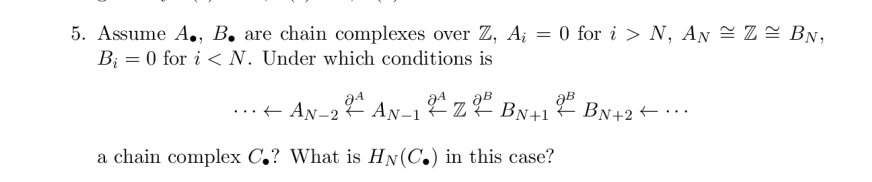
\includegraphics[]{image.png}

3. Connecting homomorphisms

Let $\epsilon: 0\ra A_* \ra B_* \ra C_* \ra 0$ a SES of chain complexes over some commutative ring $R$

\begin{itemize}
    \item Define the connecting homomorphisms $\partial :H_n(C_*)\ra H_{n-1}(A_*)$
    \item Point out two choices on which the definition depends
    \item Write down the LES of homology groups induced by $\epsilon$
    \item How is the LES of a pair $(X,X_0)$ for $X_0$ a subspace of $X$ defined?
\end{itemize}

4. Eilenberg-Steenrod axioms

\begin{itemize}
    \item Name all axioms for a homology theory $h_*(X,A)$
    \item Why does singular homology theory satisfy the dimension theorem?
    \item If $h_*^a$, $h_*^b$ are two homology theories, is $h_*=h^a_*\oplus h^b_*$ a homology theory?
\end{itemize}

5. Relative homology groups

\begin{itemize}
    \item Definte the relative homology groups of a pair of spaces $(X;A)$ 
    \item Write down the LES of a pair $(X,A)$ including the homomorphisms in this sequence
    \item Use this sequence to compute the homology of $X=F_2$, the surface of genus 2, where $A$ is the right half of $X$
\end{itemize}

6. Hurewicz isomorphism

\begin{itemize}
    \item Define the Hurewicz homomorpism in degree $1$
    \item Verify that it's well-defined and state which choices your definition depends on
    \item Formulate the Hurewicz theorem in degree $1$
    \item Prove: if map $f:(X,x)\ra (Y,y)$ induces an epimorphism $f_*$ between the fundamental groups $\pi_1$, then it also induces and epimorphism between the first homology groups. 
\end{itemize}

7. Chain maps

\begin{itemize}
    \item What is a chain map of degree $k$ between two chain complexes
    \item Prove: A chain map of degree $k$ induces homomorphism between homology groups
    \item What is a chain hojmotopy between two chain maps of degree $k$
    \item Prove: Chain homotopic chain maps induce the same homomorphism
\end{itemize}

8. Simplicial approximation theorem

\begin{itemize}
    \item Formulate the simplicial approximation theorem
    \item Prove: if $X$ is a finite polyhedron of dimension $m <n$ then any map $f:X \ra S^n$ is null-homotopic
\end{itemize}

9. Jordan-Brouwer

\begin{itemize}
    \item Formulate the Jordan-Brouwer theorem giving the homology of the complement of a $k$-sphere S embedded in $\R^n$
    \item Define the linking number $Link(S,T)$ of a $p$-sphere $S$ and a $q$-sphere $T$ disjointly embedded in $\R^n$ where $n-1 = p+q$
    \item Prove: if $T$ is isotoped inside the complement of $S$ to $T'$ then $Link(S,T)=Link(S,T')$
\end{itemize}

10. Transfer

\begin{itemize}
    \item Define the transfer homomorphism for a $2$-fold covering $\pi: X'\ra X$ in modulo $2$ homology $H_*(-;\F_2)$
    \item Investigate the LES of coverings shown in the drawing below. Calculate all relvant homology groups, calculate the connecting homomorphism for coefficients in $\F_2$
\end{itemize}

11. Bonus questions

\begin{itemize}
    \item When did Poincare develop the concept of homology groups?
    \item When did Eilenber and Steenrod formulate their axioms?
\end{itemize}

\end{document}
1. TODO: work this in
What is the relationship between topological spaces and simplicial complexes? Each simplicial complex K
 has a geometric realization |K|
 which is a topological space consisting of Euclidean simplices which are convex hulls of points in general position in some Rn
 (each combinatorial n
-simplex which is a finite set of vertices is realized as a Euclidean simplex, and these Euclidean simplices are glued together by the corresponding combinatorial incidences of the faces). But certainly not every space is the geometric realization of simplicial complex. Moreover, two non-isomorphic simplicial complexes may have homeomorphic geometric realizations - are their homology groups isomorphic ("topological invariance of simplicial homology")? It was discovered that this question cannot be answered by purely combinatorial methods. This was the origin of singular homology

2. TODO: p. 41 49 Sato work out example of simplicial homology

3. TODO: https://suess.sdf-eu.org/website/lang/de/algtop/notes4.pdf

4. TODO: https://people.reed.edu/~davidp/411/handouts/simplicial.pdf



\newpage 
\section{Ausgearbeitete Beispiele, die Spaß machen}
\subsection{Tripel-Sequenzen existieren}
Gegeben $A\subseteq B \subseteq X$, zeige, dass es eine natürliche exakte Tripel-Sequenz gibt
$$
\begin{aligned}
& \ldots \stackrel{\partial_{n+1}(X, B, A)}{\longrightarrow} \mathcal{H}_n(B, A) \stackrel{\mathcal{H}_n(i)}{\longrightarrow} \mathcal{H}_n(X, A) \stackrel{\mathcal{H}_n(j)}{\longrightarrow} \mathcal{H}_n(X, B) \\
\ldots & \stackrel{\partial_n(X, B, A)}{\longrightarrow} \mathcal{H}_{n-1}(B, A) \stackrel{\mathcal{H}_{n-1}(i)}{\longrightarrow} \mathcal{H}_{n-1}(X, A) \stackrel{\mathcal{H}_{n-1}(j)}{\longrightarrow} \mathcal{H}_{n-1}(X, B) \stackrel{\partial_{n-1}(X, B, A)}{\longrightarrow} \ldots,
\end{aligned}
$$

\subsection{Computing homology}
\begin{outline}
    A collection of usefule tricks I've seen
    \1 Excision 
    \1 Finding a subspace
    \1 Pushout
    \1 Homotopy equivalence to a point + splitting lemma
        \2 contractible $\iff$ identity null-homotopic
\end{outline}
